\chapter{Background}                                \label{Chapter:background}


% ===================================================================================================
% === NEW SECTION === NEW SECTION === NEW SECTION === NEW SECTION === NEW SECTION === NEW SECTION ===
% ===================================================================================================
\section{Transdermal drug delivery}                 \label{Chapter:background/transdermal drug delivery}
    % \subsection{Problems}                           \label{Chapter:background/transdermal drug delivery/problems}
    % \subsection{Alternative methods}                \label{Chapter:background/transdermal drug delivery/alternative methods}

    Transdermal drug delivery is a method of delivery for pharmaceutical solutions that are unsuitable for ingestion or cannot penetrate through the skin. Many vaccines and insulin are delivered by this approach\,\cite{sadrzadeh2007}. While being efficient and precise, transdermal drug delivery via hypodermic needle is time-consuming, labor intensive, and hazardous. The procedure requires the operator to attach a hollow needle to a syringe, then extract the drug, eliminate air bubbles in the syringe and sterilize the applied area thoroughly. Once prepared, the operator can slowly inject a high volume of drug. During disposal, needle stick is a safety hazard. Needle-stick injuries hold a high risk of transmitting contagious diseases such as HIV, HBV, and HCV. Percutaneous sharps injuries affected millions of individuals across the world\,\cite{pruss2005}. 
    
    Today, needle sticks and sharp objects still represent a significant challenge in creating a safe environment for professional health care practitioners. Pain\,\cite{schneider1994} and needle-phobia\,\cite{hamilton2005,Nir2003} are other motivations to develop and popularize alternative strategies.
    
    Some distinct transdermal drug delivery methods were invented to tackle issues of needle injection. They include iontophoresis\,\cite{dhote2012}, sonophoresi\,\cite{bommanan1992}, permeation enhancement by chemicals\,\cite{karande2006}, micro-needles on patch\,\cite{cormier2004}, and jet injection\,\cite{taberner2006}. 

% ===================================================================================================
% === NEW SECTION === NEW SECTION === NEW SECTION === NEW SECTION === NEW SECTION === NEW SECTION ===
% ===================================================================================================
\section{Needle-free Jet Injection}                 \label{Chapter:background/needle-free jet injection}
    
    
    % -----------------------------------------------------------------------------------
    % --- NEW SUB SECTION --- NEW SUB SECTION --- NEW SUB SECTION --- NEW SUB SECTION --- 
    % -----------------------------------------------------------------------------------
    \subsection{How it works}                       \label{Chapter:background/needle-free jet injection/how it works}
    
        \ac{NFJI}, commonly called “hypo-spray” in science fiction, was patented in 1960\,\cite{ismach1962}. Figure\,\ref{fig:chapter/background/explain needle free/original injector} shows the original \acs{NFJI} device, “Ped-O-Jet” in use for the purpose of mass vaccination\,\cite{DictionnairesetEncyclopediessurAcademic}. This device was invented  upon realizing that pressurized fluid can penetrate human skins. Fluid streams of appropriate diameter and velocity can produce sufficient pressure to breach through the skin layers up to a particular desired depth. 
        
        \begin{figure*}[!ht]
            \centering
            \subfloat[Ped-O-Jet in use]{
                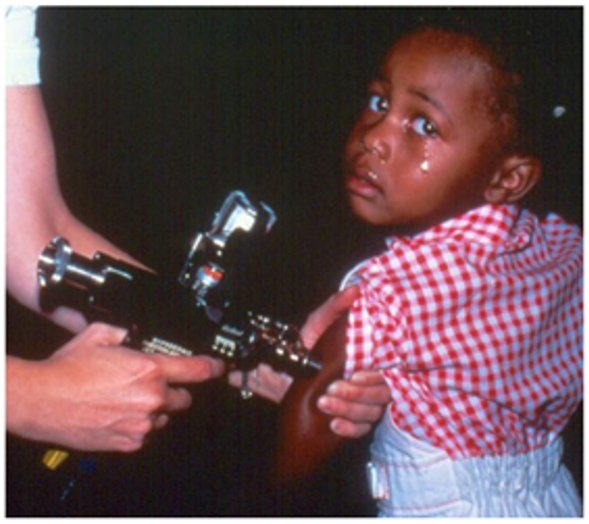
\includegraphics[width=0.35\textwidth]{chap2/images/original_injector.png}
                \label{fig:chapter/background/explain needle free/original injector}
            }
            \qquad
            \subfloat[Needle injection versus Needle-free injection]{
                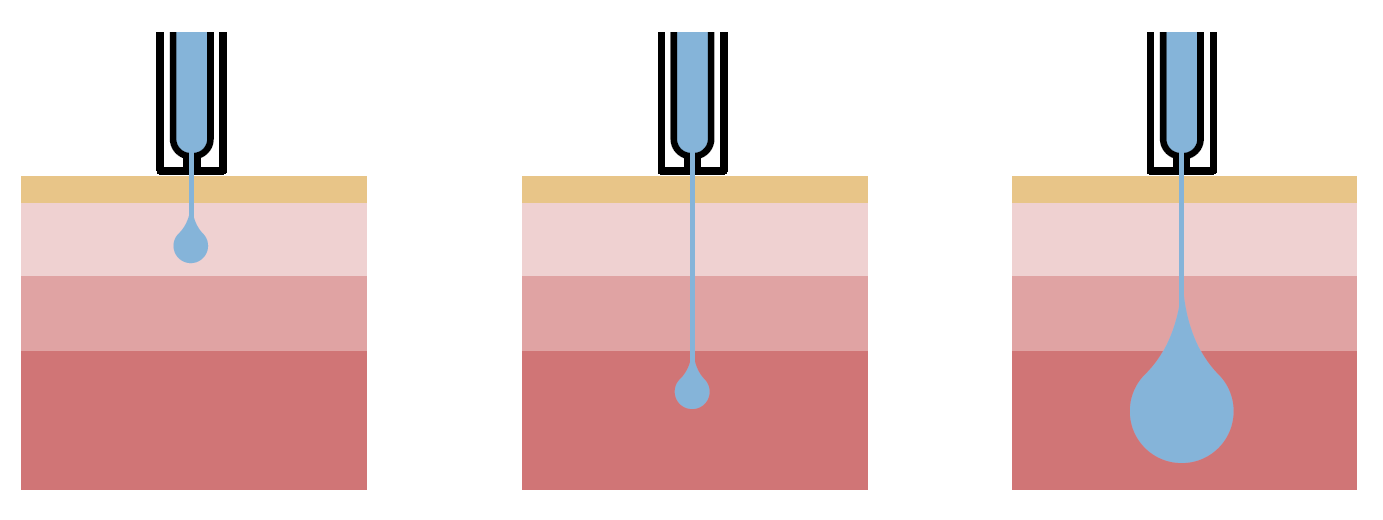
\includegraphics[width=0.45\textwidth]{chap2/images/needle_vs_needle_free.png}
                \label{fig:chapter/background/explain needle free/needle vs no needle}
            }
            \caption{
                Two different style of optimization objective function evaluation.
            }   \label{fig:chapter/background/explain needle free}
        \end{figure*}
        
        A subcutaneous or intramuscular jet injection could be realized by forcing a fluid jet of $\mathrm{76-360\,\mu m}$  diameter to penetrate the human skin at a speed faster than $\mathrm{100 m/s}$\,\cite{mitragotri2006,Hogan2006}. Figure\,\ref{fig:chapter/background/explain needle free/needle vs no needle} shows that an ideal jet injection would deliver the drug in a similar manner to which of a hypodermic needle injection\,\cite{InsuJet2013}.
        
        % Even though this method adopts the use of needle-free apparatus, biological material can still be unwillingly transferred if there are no appropriate decontamination schemes. Concerns have been raised in the literature about potential transmission of blood-borne infections by multiple-use \acs{NFJI} since the early 1970s\,\cite{kremer1970, weintraub1988}. Figure\,\ref{fig:chapter/background/injection mechanism} illustrates three possible mechanisms of how blood contamination can take place\,\cite{hoffman2001}. 
        
        % \begin{figure*}[!ht]
    
        %     \centering
        %     \subfloat[]{
        %         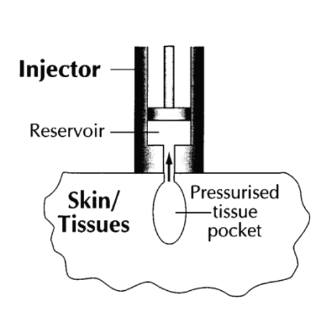
\includegraphics[width=0.29\textwidth]{chap2/images/jet_injection_mechanism_1.png}
        %         \label{fig:chapter/background/injection mechanism/1}
        %     }
        %     \subfloat[]{
        %         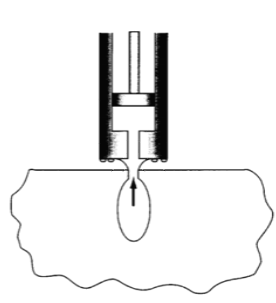
\includegraphics[width=0.25\textwidth]{chap2/images/jet_injection_mechanism_2.png}
        %         \label{fig:chapter/background/injection mechanism/2}
        %     }
        %     \subfloat[]{
        %         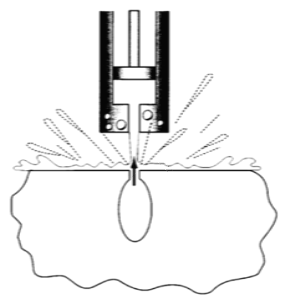
\includegraphics[width=0.27\textwidth]{chap2/images/jet_injection_mechanism_3.png}
        %         \label{fig:chapter/background/injection mechanism/3}
        %     }
        %     \caption{
        %         3 possible mechanisms of blood contamination in ‘mass campaign jet injectors’. 
        %     }   \label{fig:chapter/background/injection mechanism}
        % \end{figure*}    
        
        % Scenario in Figure\,\ref{fig:chapter/background/injection mechanism/1} shows that tissues return fluid into the reservoir as injection pressure diminishes. Liquid flows out to the tip of the injector as the injector’s tip is removed from the applied area as illustrated in Figure\,\ref{fig:chapter/background/injection mechanism/2}. Scenario in Figure\,\ref{fig:chapter/background/injection mechanism/3} displays a ‘splash back’ of jet stream during injection. Uninterrupted, continuous, reuse of \acs{NFJI} has historically caused instances of mass HBV spread\,\cite{canter1990}. For prevention of future mass infection, ‘mass campaign jet injectors’ were disapproved for human use by the World Health Organization\,\cite{who2005}. Nowadays, reusable \acsp{NFJI} for human use must accommodate replaceable syringes. 
    
    
    % -----------------------------------------------------------------------------------
    % --- NEW SUB SECTION --- NEW SUB SECTION --- NEW SUB SECTION --- NEW SUB SECTION --- 
    % -----------------------------------------------------------------------------------
    \subsection{Underlying mechanics}               \label{Chapter:background/needle-free jet injection/underlying mechanics}
    
        \begin{figure*}[!ht]
            \centering
            \subfloat[]{
                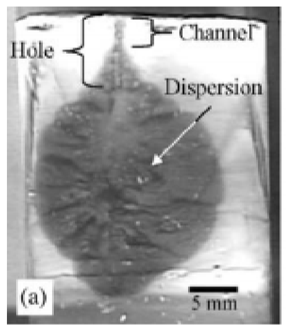
\includegraphics[width=0.28\textwidth]{chap2/images/jet_injection_mechanics_1.png}
                \label{fig:chapter/background/underlying mechanics/1}
            }
            \quad
            \subfloat[]{
                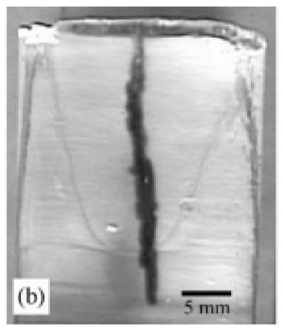
\includegraphics[width=0.28\textwidth]{chap2/images/jet_injection_mechanics_2.png}
                \label{fig:chapter/background/underlying mechanics/2}
            }
            \quad
            \subfloat[]{
                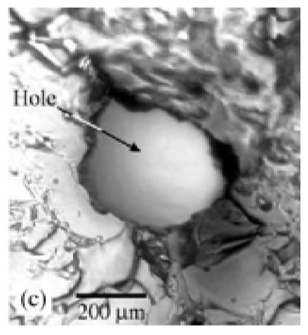
\includegraphics[width=0.3\textwidth]{chap2/images/jet_injection_mechanics_3.png}
                \label{fig:chapter/background/underlying mechanics/3}
            }
            \caption{
                (a) The general shape of jet penetration into polyacrylamide gel; (b) Side view of the same gel sample; (c) The transverse slice of the gel shows the presence of the cylindrical channel.
            }   \label{fig:chapter/background/underlying mechanics}
        \end{figure*}
    
        To explore mechanics of NFJI into the skin, Schramm-Baxtex et al.\,\cite{Schramm-Baxter2004b} conducted an experiment where a high-speed camera monitored a spring-driven jet injection into polyacrylamide gel as a test bed as shown in Figure\,\ref{fig:chapter/background/underlying mechanics}. Motion analysis demonstrated the presence of three distinct jet injection phases: erosion, stagnation, and dispersion. The erosion phase is the period when jet penetrates in the form of a cylindrical channel. The brief reduction of upfront kinetic energy causes the fluid to start building up at a certain depth, described as the stagnation phase. The dispersion phase is where a drug volume infiltrates the cracks propagated within the gel by fluid pressure during previous phases. The maximum depth was controlled by altering the jet velocity at erosion, and likewise, the amount of drug delivered is determined in by the jet speed at the dispersion phase\,\cite{Stachowiak2009}.
        
        
        \begin{figure*}[!ht]
            \centering
            \subfloat[]{
                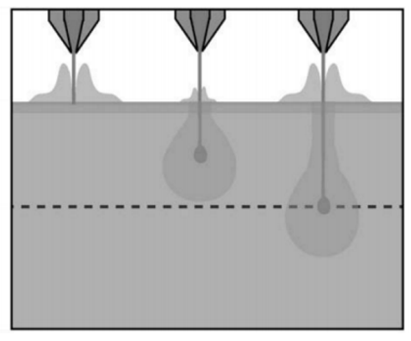
\includegraphics[width=0.515\textwidth]{chap2/images/1_speed_injection.png}
                \label{fig:chapter/background/2 speeds mechanics/just 1 speed}
            }
            \qquad
            \subfloat[]{
                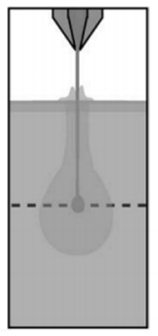
\includegraphics[width=0.20\textwidth]{chap2/images/2_sppeds_injection.png}
                \label{fig:chapter/background/2 speeds mechanics/2 speeds}
            }
            \caption{
                Need for temporal control of jet velocity in needle-free transdermal drug delivery: (a) constant low-velocity delivery (left), medium-velocity delivery (center), and high-velocity delivery (right); (b)Desired drug delivery showing sufficient penetration depth and minimal pooling. Dotted line represents the desired depth of injection.
            }   \label{fig:chapter/background/2 speeds mechanics}
        \end{figure*}
        
        
        Difficulty in controlling depth injection and ‘splash back’ was the result of using a single jet velocity\,\cite{schramm2002}. Figure\,\ref{fig:chapter/background/2 speeds mechanics/just 1 speed} explains the need for temporal control of jet velocity in needle-free transdermal drug delivery: (a) constant low-velocity delivery (left), medium-velocity delivery (center), and high-velocity delivery (right); (b)Desired drug delivery showing sufficient penetration depth and minimal pooling. Dotted line represents the desired depth of injection[35]. At constant low pressure, the jet may not penetrate into the skin (left), while constant, medium-pressure jet velocity may breach the skin with minimal ‘splash back’, yet reach an insufficient depth (middle).A high-pressure stream may reach the desired depth, but fluid pooling cannot be avoided (right). With the use of an initial high jet pressure followed by a lower holding pressure, it was predicted that ’splash back’ would be reduced while the jet disperses at the correct depth\,\cite{wendell2006}. This concept is portrayed in Figure\,\ref{fig:chapter/background/2 speeds mechanics/2 speeds}. Taberner et al.\,\cite{taberner2012} demonstrated that the use of a high degree of fluid stream velocity control can deploy this strategy reliably.
    
    
    % -----------------------------------------------------------------------------------
    % --- NEW SUB SECTION --- NEW SUB SECTION --- NEW SUB SECTION --- NEW SUB SECTION --- 
    % -----------------------------------------------------------------------------------
    \subsection{Commercially available options}     \label{Chapter:background/needle-free jet injection/commercially available options}
        
        Commercially available \acsp{NFJI} including BIOJECT Zeajet\footnote{http://www.bioject.com/products/zetajet-info} , INJEX 30\footnote{https://www.injex.com.au/injex/injex} , PHARMAJET Stratis\footnote{http://pharmajet.com/fda-approved-needleless-flu-shot} , COMFORT-IN\footnote{http://www.comfort-in.com/diabetes.html}  are spring-powered, small, portable, and handheld devices. They are capable of delivering either vaccination or insulin in a small dose, with volume limited to $\mathrm{300\,\mu L}$. Figure\,\ref{fig:chapter/background/pharma jet stratis} illustrates the appearance, construction, and mechanism of the spring-loaded PHARMAJET Stratis NFJI as an example. These devices come in various shapes, sizes, injection volumes, and target skin layers. However, their primary structure consists of three main components:
        \begin{itemize}
            \item Energy storage - compressed gas, spring coil or explosives\,\cite{taberner2012}, which are often accompanied by a recharging device,
            \item Piston - actuator with various size and triggering method to accomplish desired pressure profile as well as injection volume specification,
            \item Replaceable syringe - single use container with orifice hole diameter of under $\mathrm{1\,mm}$.
        \end{itemize}
        
        \begin{figure*}[!ht]
            \centering
            \subfloat[\acs{NFJI} device and replaceable syringe]{
                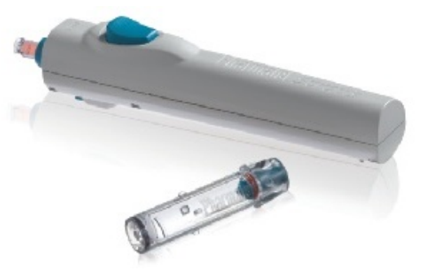
\includegraphics[width=0.40\textwidth]{chap2/images/pharma_jet_stratis.png}
                \label{fig:chapter/background/pharma jet stratis/full view}
            }
            \qquad
            \subfloat[Spring loaded mechanism of the device]{
                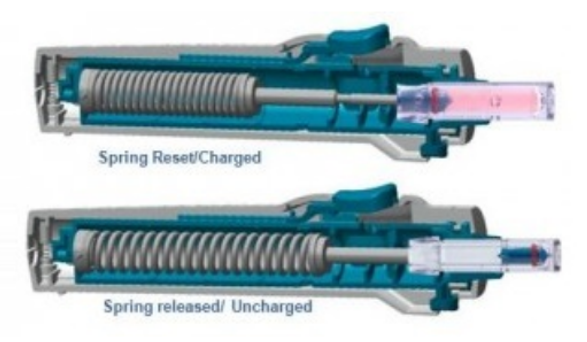
\includegraphics[width=0.45\textwidth]{chap2/images/pharma_jet_stratis_cut_view.png}
                \label{fig:chapter/background/pharma jet stratis/cut view}
            }
            \caption{
                SUNFJI Pharma Jet Stratis™ from PharmaJet™
            }   \label{fig:chapter/background/pharma jet stratis}
        \end{figure*}
        
        Once triggered, stored energy produces varying pressure on the injection cylinder until the piston reaches the end of its track. Different devices utilize different recoil or trigger mechanisms, but no system is capable of monitoring and measuring injection performance. Instead of concentrated fluid delivery in a narrow stream down the tissue, these devices tend to spread the drug content in a cone shape\,\cite{baxtex2005}. Figure\,\ref{fig:chapter/background/jet injection effectiveness/mechanical devices pressure curve} shows the sharp peak and oscillating nature of the pressure produced by injection stream of a BIOJECT Vitajet 3™ spring powered \acsp{NFJI}\,\cite{schramm2002}. Schneider et al.\,\cite{schneider1994} reported that without stroke velocity and position control, the sharp fluid pressure profile peak could cause pain, bruises, bleeding, and blisters. Their studies also showed evidence that the same spring powered NFJI device exhibits inconsistent performance across different skin types and conditions. 
        
        Despite being a safer alternative, mechanically powered \acsp{NFJI} require manual recharging. Thus, the average cycle time was recorded to be no faster than that of a conventional hypodermic needle injection\,\cite{PharmaJet2011}. More advanced \acsp{NFJI} like LECTRAJET  have shown the capability of automatic spring recoil to reduce reload time. Lack of pressure control, low injection volume (typically $0.05$ to $0.3\,\mathrm{mL}$), long cycle time, poor repeatability and reproducibility are drawbacks of commercially available mechanically powered \acsp{NFJI}.
        
        \begin{figure*}[!ht]
            \centering
            \subfloat[Typical pressure curve for a $152\,\mathrm{\mu m}$ diameter nozzle from injector Vitajet\,3™]{
                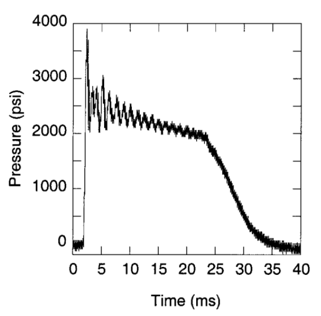
\includegraphics[width=0.43\textwidth]{chap2/images/jet_injection_pressure_curve.png}
                \label{fig:chapter/background/jet injection effectiveness/mechanical devices pressure curve}
            }
            \qquad
            \subfloat[Delivery of mannitol by jet injection into human (A), porcine abdominal (B), and porcine dorsal skin (C) using the same device at $177\,\mathrm{m/s}$. There is a significant difference between each type of skin tested ($p=0.001$)]{
                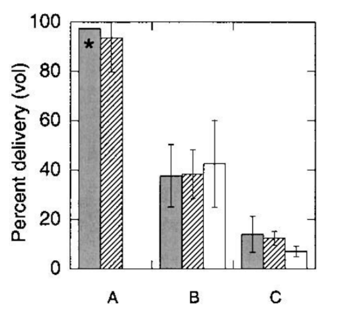
\includegraphics[width=0.45\textwidth]{chap2/images/jet_injection_delivery_study.png}
                \label{fig:chapter/background/jet injection effectiveness/delivery statistic}
            }
            \caption{
                Results of different jet injection study on mechanically powered \acs{NFJI} devices demonstrating rough pressure profile and poor adaptability.
            }   \label{fig:chapter/background/jet injection effectiveness}
        \end{figure*}


    % -----------------------------------------------------------------------------------
    % --- NEW SUB SECTION --- NEW SUB SECTION --- NEW SUB SECTION --- NEW SUB SECTION --- 
    % -----------------------------------------------------------------------------------
    \subsection{Controllable \acs{NFJI} devices}    \label{Chapter:background/needle-free jet injection/Controllable NFJI}
    
        Recent achievements in high power density actuators enabled successful prototypes of electronic controlled \acsp{NFJI} which were capable of real-time jet velocity control. Hemond et al. [24] suggests four advantages of electronics control over traditional needle injection and mechanically powered jet injection:
        
        \begin{itemize}
            \item Controllable - capable of maintaining high pressure without the need of trading-off for injection volume,
            \item Reliable - capable of producing consistent jet pressure on a broad range of skin properties and different injection types,
            \item Versatile - automatic reload under closed loop control or injection volume control,
            \item Measurable - convenient in monitoring progress to evaluate the performance of injection.
        \end{itemize}
        
        This class of device performs injections by utilizing different electrically powered actuators: dynamically controlled piezo-electric actuators\,\cite{Stachowiak2009}, laser pulsed microjets\,\cite{tawaga2013, park2012} and Lorentz force voice coil motors\,\cite{taberner2006,hemond2006}. Piezo-electric and laser pulse methods are limited to sub $\mathrm{\mu L}$ injections. Scaling of Piezo-electric technology to   range in injection volume appear ambitious. Cumbersome ‘off-the-shelf’ voice coil actuators which will be explored in \ref{Chapter:background/voice coil motors for NFJI} are not yet suitable to become handheld.

% ===================================================================================================
% === NEW SECTION === NEW SECTION === NEW SECTION === NEW SECTION === NEW SECTION === NEW SECTION ===
% ===================================================================================================
\section{Voice coil motors for \acs{NFJI}}          \label{Chapter:background/voice coil motors for NFJI}
    
    
    % -----------------------------------------------------------------------------------
    % --- NEW SUB SECTION --- NEW SUB SECTION --- NEW SUB SECTION --- NEW SUB SECTION --- 
    % -----------------------------------------------------------------------------------
    \subsection{Principle of operation}             \label{Chapter:background/voice coil motors for NFJI/principle}


    The \ac{VCM} is a type of Lorentz-force actuator. \ac{VCM} can either have the magnet or the coil as moving part. Figure\,\ref{fig:chapter/background/vcm cut view} presents the construction of moving coil configuration\,\cite{taberner2006}. Here, a Nd-Fe-B magnet is used to generate the magnetic field. The magnet is placed between a steel top plate and the steel casing to direct the flow of magnetic flux in a contained loop. In between the top plate and steel case is a region of air gap that allows of copper winding to slide up or down. Linear force $F$ is proportional to strength of the magnetic field $B$ through wire, and the electric current per unit area $J$ passing through the coil:
    
    
    \begin{equation}
        F=J\times B
        \label{eq:force produce via field and current}
    \end{equation}

    The polarity of the current also dictates which direction the coil will move. It is clear that more force can be generated by either strengthening the magnetic field or increasing the current through the coil. Adjusting other parameters such as coil geometry, coil thickness, magnet materials, and aspect ratio can alter the motor force constant and stroke length.
    
    
    \begin{figure}[!ht]
      \centering
      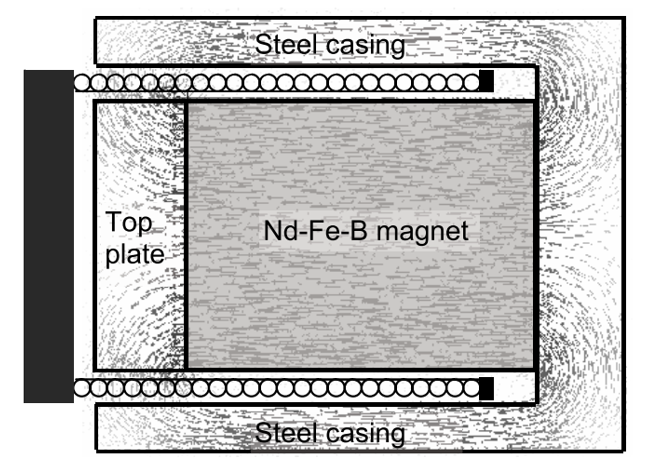
\includegraphics[width=0.5\textwidth]{chap2/images/vcm_cut_view.png}
      \caption{Construction of a voice coil motor with moving coil.}
      \label{fig:chapter/background/vcm cut view}
    \end{figure}
    
    
    % -----------------------------------------------------------------------------------
    % --- NEW SUB SECTION --- NEW SUB SECTION --- NEW SUB SECTION --- NEW SUB SECTION --- 
    % -----------------------------------------------------------------------------------
    \subsection{Application to \acs{NFJI}}          \label{Chapter:background/voice coil motors for NFJI/application}
    
    
    Recently, collaboration between the \ac{MIT} and \ac{ABI} Bioinstrumentation Labs has created two prototypes jet injectors actuated by customized Lorentz-force \ac{VCM}\,\cite{taberner2006,ruddy2014} shown in Figure\,\ref{fig:chapter/background/vcm injectors}. With the use of real-time feedback control, these systems have demonstrated highly controllable and repeatable injections against a broad range of different test tissues, depths, and dosage volumes\,\cite{taberner2012}. With the successful prototypes, the vision was to advance the prototypes into portable and high volume injector devices.


    \begin{figure*}[!ht]
        \centering
        \subfloat[]{
            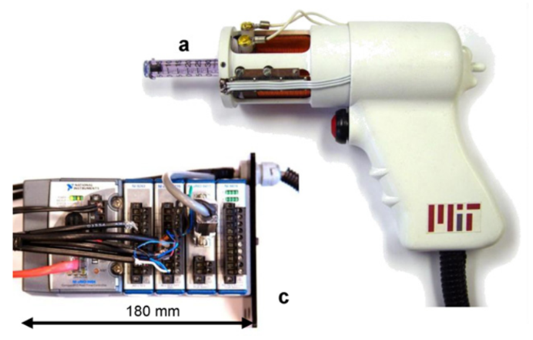
\includegraphics[width=0.5\textwidth]{chap2/images/vcm_taberner2006.png}
            \label{fig:chapter/background/vcm injectors/taberner2006}
        }
        \qquad
        \subfloat[]{
            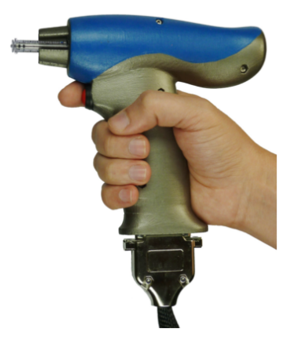
\includegraphics[width=0.28\textwidth]{chap2/images/vcm_ruddy2014.png}
            \label{fig:chapter/background/vcm injectors/ruddy2014}
        }
        \caption{
            Lorentz-force \acs{VCM} actuated \ac{NFJI}: Handheld injector and cRIO controller system (a); Hand-held injector and charged capacitor amplifier/controller system (b).
        }   \label{fig:chapter/background/vcm injectors}
    \end{figure*}
    
    
    \begin{figure}[!ht]
      \centering
      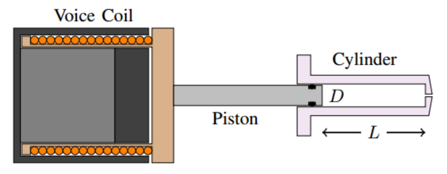
\includegraphics[width=0.6\textwidth]{chap2/images/vcm_for_nfji.png}
      \caption{A basic schematic of a voice coil actuated \acs{NFJI}. $L$ and $D$ are the cylinder’s working length (stroke length) and diameter, respectively.}
      \label{fig:chapter/background/vcm for nfji}
    \end{figure}
    
    
    Figure\,\ref{fig:chapter/background/vcm for nfji} shows a basic schematic of a voice coil actuated \acs{NFJI}. $L$ and $D$ are the cylinder’s working length (stroke length) and diameter, respectively\,\cite{ruddy2014}. In this device, injection volume can be enlarged by either up-scaling the ampoule diameter $D$, or the working stroke length $L$, or both. A jet injector with an ampoule diameter $D$ requires an actuation force $F$ to be provided by the motor. For constant peak jet velocity $v_{jet}$ and fluid density $\rho$:
    
    
    \begin{equation}
        F=\frac{\pi}{8}\rho {v_{jet}}^2 D^2
        \label{eq:force produce relationship in motor powered NFJI}
    \end{equation}
    
    
    If syringe’s diameter\,$D$ is chosen to scale with injection volume, electric power\,$P$ needs to scale with the square of $D$’s scaling ratio due to the relationship:
    
    
    \begin{equation}
        P=F v_{piston}
        \label{eq:power required for F and v_piston}
    \end{equation}
    
    
    where $v_{piston}$ is the speed of the moving piston. If syringe’s diameter  is chosen to scale with injection volume, electric power\,$P$ needs to scale with the square of $D$’s scaling ratio. Given that the jet velocity follows the varying velocity strategy explained in Section\,\ref{Chapter:background/needle-free jet injection/underlying mechanics}, the motor needs to achieve the peak jet velocity required for the brief erosion phase, then the lower jet velocity speed for dispersion phase. For only for a very short period, the device is required to produce much more power than its average power drawn. It is not common to find energy storage and powering devices at power magnitude of many kilowatts, provided in a portable fashion.
    
    
    % -----------------------------------------------------------------------------------
    % --- NEW SUB SECTION --- NEW SUB SECTION --- NEW SUB SECTION --- NEW SUB SECTION --- 
    % -----------------------------------------------------------------------------------
    \subsection{Scaling properties and limitations} \label{Chapter:background/voice coil motors for NFJI/scaling and limitation}
    
    
    The following key relationship relates the power dissipation on the motor winding $P$, density of fluid to be deliver $rho$, ampoule volume $V$, jet velocity $v$, motor constant $K_m$, and distance travelled by the piston stroke $L$ \cite{Williams2012}:
    
    
    \begin{equation}
        P=\frac{\rho^2 V^2 {v_{jet}}^4}{4 K_m L^2}
        \label{eq:power required for F,V,v_jet,K_m, and L}
    \end{equation}
    
    
    To compare the force exerted over power consumed in different motors, the motor constant $K_m$ measured in $\mathrm{N/\sqrt{W}}$  is typically used. Note that this relationship is true of all direct drive linear motors, which apply force directly to single injection ampoule without any mechanical coupling transmission.
    
    
    Utilizing a general scaling magnetic and thermal model made for steady-state force production of \ac{PMLSM} constructed by Ruddy et al.\,\cite{Ruddy2011DesignMotors}, an optimal \acs{VCM} hand-piece was built to deliver $\mathrm{300\,\mu L}$ of the drug over a $\mathrm{50\,ms}$ period\,\cite{taberner2006}. The peak power required for this procedure was as high as 10 kW to produce peak force of $\mathrm{300\,N}$ of over the stroke length of $\mathrm{35\,mm}$. Due to the extremely short duration of the force profile, the heat generated is far from enough to cause permanent demagnetization in the permanent magnet array; thus, the motor design neglect heat transfer. In the same body of work, the authors pointed out that scaling laws of voice coil actuator fit for needle free injection means that the power $P$ required and motor mass $M$ both grow faster than injection volume $V$:
    
    
    \begin{equation}
        M \propto V^{6/5}
        \label{eq:scaling property of VCM}
    \end{equation}


    While the potential of using \acsp{VCM} in portable \acs{NFJI} devices has been proven, this type of motor is power inefficient. Without breakthrough improvements, \acsp{VCM} pose a considerable restriction on the portability of the electronics control system, as well as the size of the injector handpiece motor. Based on the model presented in that work, a \acs{VCM} with mass of over $\mathrm{1\,kg}$ is required to deliver $\mathrm{1\,mL}$. Thus, it was impractical to use a direct-drive linear \acsp{VCM} to deliver regular livestock injections, where the volume can be as high to $\mathrm{10\,mL}$. 

% ===================================================================================================
% === NEW SECTION === NEW SECTION === NEW SECTION === NEW SECTION === NEW SECTION === NEW SECTION ===
% ===================================================================================================
\section{Linear synchronous motors for NFJI}        \label{Chapter:background/linear synchronous motors for NFJI}
    \subsection{Classification}                     \label{Chapter:background/linear synchronous motors for NFJI/classification}
    \subsection{Advantages}                         \label{Chapter:background/linear synchronous motors for NFJI/advantages}
    \subsection{Challenges}                         \label{Chapter:background/linear synchronous motors for NFJI/challenges}


% ===================================================================================================
% === NEW SECTION === NEW SECTION === NEW SECTION === NEW SECTION === NEW SECTION === NEW SECTION ===
% ===================================================================================================
\section{Electromagnetic field theory}              \label{Chapter:background/electromagnetic field theory}
    \subsection{Quasi-static Maxwell equations}     \label{Chapter:background/electromagnetic field theory/quasi-static maxwell equations}
    \subsection{Ferromagnetic materials}            \label{Chapter:background/electromagnetic field theory/ferromagnetic materials}
    \subsection{Materials for motor construction}   \label{Chapter:background/electromagnetic field theory/materials for motor construction}


% ===================================================================================================
% === NEW SECTION === NEW SECTION === NEW SECTION === NEW SECTION === NEW SECTION === NEW SECTION ===
% ===================================================================================================
\section{Modelling techniques for motors}           \label{Chapter:background/modelling techniques for designing motors}
    \subsection{Numerical methods}                  \label{Chapter:background/modelling techniques for designing motors/numerical methods}
    \subsection{Analytical methods}                 \label{Chapter:background/modelling techniques for designing motors/analytical methods}
    \subsection{Semi-analytical methods}            \label{Chapter:background/modelling techniques for designing motors/semi-analytical methods}
    \subsection{Empirical methods}                  \label{Chapter:background/modelling techniques for designing motors/empirical methods}


% ===================================================================================================
% === NEW SECTION === NEW SECTION === NEW SECTION === NEW SECTION === NEW SECTION === NEW SECTION ===
% ===================================================================================================
\section{Optimization methods}                      \label{Chapter:background/optimization methods}
    \subsection{Classification}                     \label{Chapter:background/optimization methods/classification}
    \subsection{Application in motor design}        \label{Chapter:background/optimization methods/application in motor design}


% ===================================================================================================
% === NEW SECTION === NEW SECTION === NEW SECTION === NEW SECTION === NEW SECTION === NEW SECTION ===
% ===================================================================================================
\section{Summary}                                   \label{Chapter:background/summary}